\begin{frame}{Fazit: Modellqualität}
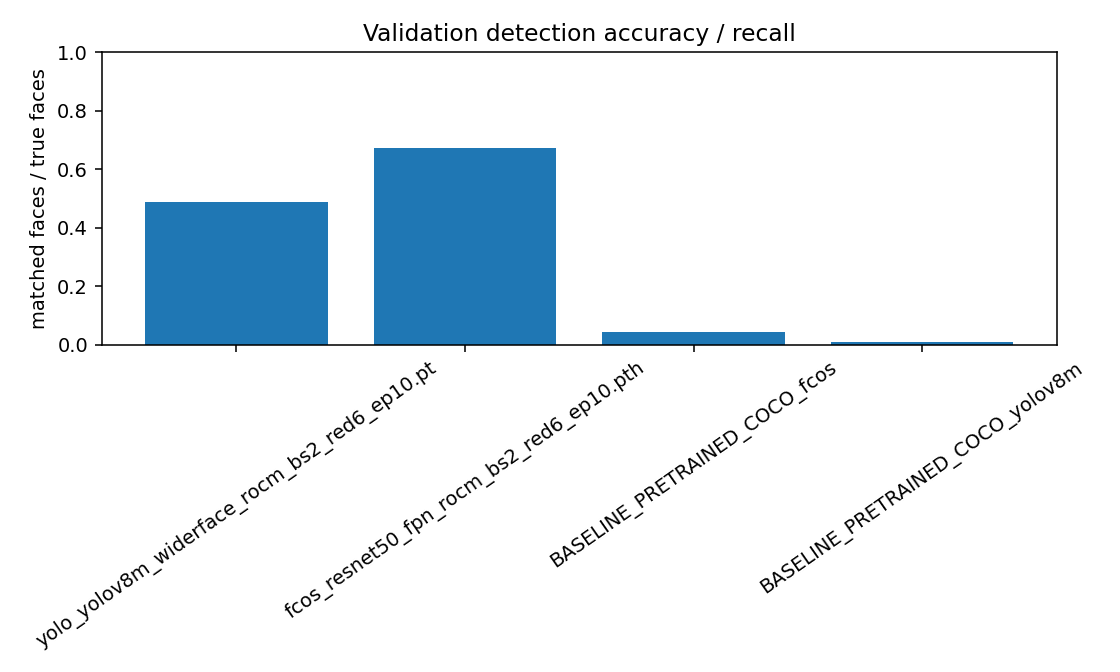
\includegraphics[width=\textwidth,height=0.50\textheight,keepaspectratio]{imglib/face_model_lab/red6_validation_recall.png}
\vspace{0.2em}
\small
\begin{itemize}
    \item FCOS red6 ep10 erreicht den besten Recall: 0,673 auf 500 Bildern mit 5.015 GT-Faces.
    \item COCO-Baselines fallen klar ab und bestätigen die Notwendigkeit von Face-Finetuning.
\end{itemize}
\end{frame}

\begin{frame}{Fazit: Pipeline-Entscheidung}
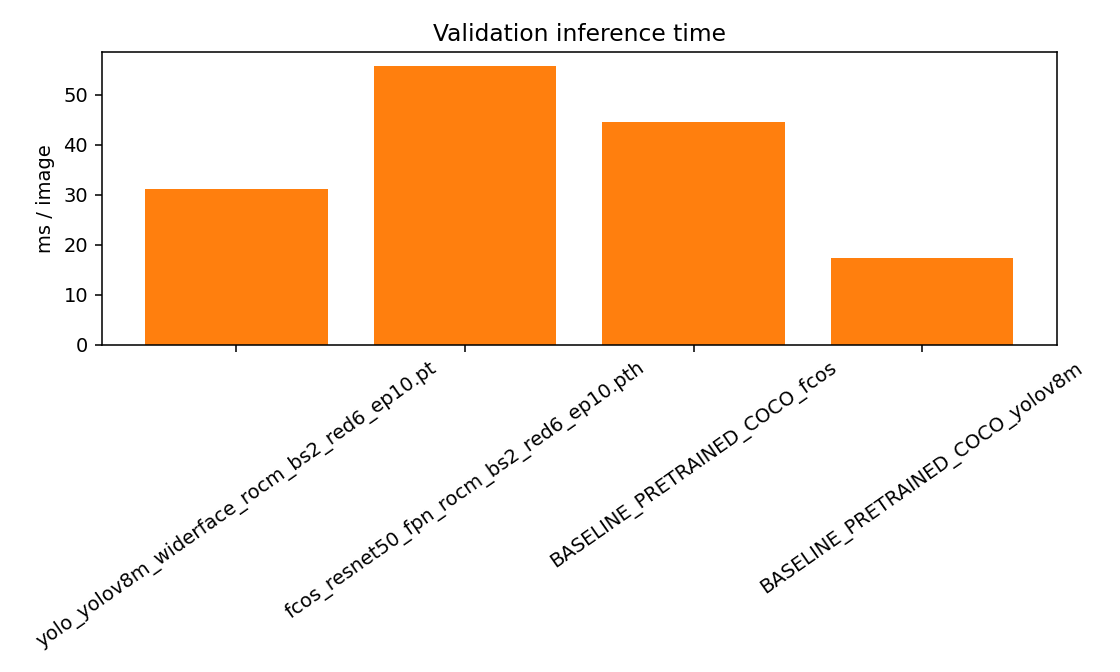
\includegraphics[width=\textwidth,height=0.50\textheight,keepaspectratio]{imglib/face_model_lab/red6_validation_latency.png}
\vspace{0.2em}
\small
\begin{itemize}
    \item YOLOv8m red6 ep10 erreicht Recall 0,488, ist aber schneller und pipelinefreundlicher.
    \item Für Datenschutz zählt zuerst Abdeckung; für die praktische Video-Pipeline zählen zusätzlich Geschwindigkeit und Artefakte.
\end{itemize}
\end{frame}
